\documentclass[12p]{article}
\usepackage{a4wide} %strona formatu a4, szeroko wypełniona tekstem
\usepackage{amsmath} %dodatkowe komendy, np. \underset
\usepackage{polski} %polskie litery
\usepackage{graphicx} 
\usepackage{amssymb}
\usepackage{tikz}
\usepackage{float}
\usepackage{lmodern}
\usepackage{amsmath}
\usepackage{array}
\usepackage{makecell}
\usetikzlibrary{fit}
\usetikzlibrary{arrows}
\usepackage{tikz}
\usetikzlibrary{shapes.geometric, arrows}
\linespread{1.3}
\usepackage{geometry} 
\newgeometry{tmargin=3cm, bmargin=3cm, lmargin=4.0cm, rmargin=2.5cm}
\tikzstyle{prostokat} = [rectangle, rounded corners, minimum width=3cm, minimum height=1cm,text centered, draw=black]
\tikzstyle{arrow} = [thick,->,>=stealth]

\begin{document}

\tableofcontents
\newpage
\part{Część teoretyczna}
\section{Cel i zakres pracy}


\quad Celem pracy jest przedstawienie algorytmów kryptograficznych oraz możliwych ataków. Następnie implementacja 2 algorytmów na systemie wbudowanym oraz porównanie ich wydajności w zależności od rozmiaru szyfrowanych danych.
%2. Na początku powinien być rozdział pt. "Cel i zakres pracy", zazwyczaj krótki maksymalnie do dwóch stron, w którym powinien znaleźć się (a) cel pracy - krótko powód podjęcia się tej tematyki, ze wskazaniem na to co pracę wyróżnia na tle prac innych o podobnej tematyce, (b) zakres pracy - czyli coś na zasadzie: praca składa sie z części teoretycznej, będącej wprowadzeniem do ...., części praktycznej w której zaprezentowane własne implementacje. Później też mozna dodać: W rozdziale 1 jest to i to, rozdział 2 poświęcono ...
%Po przeczytaniu tego rozdzialu powinno być wiadomo mniej więcej jaki jest własny wkład, dlatego tak ważne jest podkreślenie znaczenia części praktycznej. Część ta pełni rolę abstraktu.

!!!!!!!!!!!!! będzie więcej opisu !!!!!!!!!!!!!!!!

\newpage
\section{Kryptografia}
%-----------------------------------
%	Rozdział 1
%-----------------------------------
\subsection{Wprowadzenie}

\quad W obecnych czasach dużym zainteresowaniem cieszy się bezpieczeństwo cybernetyczne, którego szczególną częścią jest kryptografia. Szczególnie ważne zastosowanie znajduje w branży informatycznych, militarnej, urzędach, grupach developerskich czy bankowości. Kryptografia pojawiła się znaczniej wcześniej niż platformy obliczeniowe, zainteresowali się nią już ludzie z czasów starożytnych, pojawiła się wraz z umiejętnością pisania. Powodem istnienia kryptografii jest bezpieczne i prywatne dostarczanie wiadomości. Znajduje szczególne zastosowanie w przypadku danych przesyłanych drogą internetową, dzięki kryptografii możliwe jest zapewnienie bezpieczeństwa cybernetycznego przesyłanych danych. W zależności od stopnia poufności informacji, którą chcemy zaszyfrować, aby niepożądane osoby jej nie odczytały można zastosować odmiennych algorytmów szyfrowania. 

\quad Kryptologia to połączenie kryptografii i kryptoanalizy. W języku greckim 'kryptos' oznacza ukryty, zaś 'logos' tłumaczone jest jako słowo. Kryptologia jest dziedziną zajmującą się ukrywaniem tekstu jawnego. Kryptografia jest dziedziną węższą od kryptologii, jest badaniem technik matematycznych związanych z bezpieczeństwem informacji. Do bezpieczeństwa danych można zaliczyć poufność informacji, uwierzytelnienie użytkowników i pochodzenia danych, a także integralność danych. Słowo kryptologia składa się z dwóch greckich słów: 'kryptos' znaczący ukryty i 'graph' oznaczający pisanie, jest to nauka o zabezpieczaniu danych. Za pomocą technik kryptograficznych możliwe jest zaszyfrowanie jawnego tekstu, w taki sposób aby niepożądana osoba nie mogła ich odczytać. Drugą gałęzią kryptologii jest kryptoanaliza, która zajmuje się analizą i możliwymi sposobami odszyfrowania kodu kryptograficznego.

\subsection{Powszechne ataki}
\quad W większości metod tunelowania wykorzystano szyfrowanie, które można podzielić na symetryczne i asymetryczne. Proces szyfrowania polega na przekształceniu tekstu jawnego w tekst zaszyfrowany. Szyfrowanie asymetryczne odbywa się przy użyciu dwóch kluczy: publicznego i prywatnego. Klucz publiczny jest wykorzystywany do szyfrowania danych, zaś klucz prywatny do ich odszyfrowywania. W przypadku szyfrowania symetrycznego wykorzystywany jest jeden klucz, co prowadzi do mniejszego bezpieczeństwa szyfrowania kosztem szybszego procesu szyfrowania i odszyfrowywania danych. 
Długość klucza określana jest w bitach. Dla klucza o mniejszej długości proces szyfrowania i odszyfrowywania przebiega szybciej. Wadą jest mniejsze bezpieczeństwo przesyłanych danych. Powszechnie w przypadku szyfrowania asymetrycznego nie stosuje się kluczy krótszych niż 4096 bitów. VPN umożliwia uwierzytelnienie urządzenia, sprawdzenie integralności pakietów i szyfrowanie, dzięki czemu ataki są bardziej czasochłonne i trudniejsze dla atakującego. Aby przed atakami się odpowiednio chronić warto poznać najpowszechniejsze typy ataków. Wyróżniono trzy główne metody atakowania prywatnych sieci wirtualnych :
\begin{itemize}
\item podsłuch
\newline Najpowszechniejszą metodą ataku jest podsłuchiwanie przesyłanych wiadomości przez osobę trzecią podczas wysyłania wiadomości między dwoma osobami. Niektóre protokoły i aplikację takie jak POP,FTP, TFTP, HTTP czy TELNET są narażone na ataki metodą podsłuchu. Prywatne dane takie jak nazwa użytkownika i hasło są przesyłane w postaci tekstu między dwoma urządzeniami przy użyciu wymienionych powyżej protokołów, narażając prywatne dane na łatwe ich przechwycenie poprzez niepożądaną osobę. Głównym założeniem stworzenia protokołów POP, SMTP czy Telnet było umożliwienie komunikacji poprzez Internet  z minimalnym uwierzytelnieniem użytkownika w celu zweryfikowania jego tożsamości. Głównym narzędziem do analizowania wysyłanych danych jest analizator protokołów. Pakiety wysyłane między urządzaniem źródłowym, a docelowym atakujący może przechwycić, gdy będzie miał dostęp do połączenia, które się odbywa między nimi. W celu lepszego zabezpieczenia pakietów przesyłanych przy użyciu protokołów z minimalnym uwierzytelnieniem dodano drugie uwierzytelnienie, które minimalizuje możliwości ataków przy użyciu analizatora protokołów. Przykładem z podwójnym uwierzytelnieniem będą operacje bankowe, które po podaniu loginu i hasło przy wykonywaniu danej operacji wymagają podania jednorazowego hasła, które zostało wysłane do nas elektronicznie lub drogą pocztową. Innym stosowanym rozwiązaniem jest połączenie protokołu  HTTP i SSL czy VPN i szyfrowania. Najrzetelniejszym rozwiązaniem chroniącym przed podsłuchiwaniem będzie VPN połączone z szyfrowaniem, które uniemożliwi odczytanie wysyłanej wiadomości poprzez wirtualną prywatną sieć przez osoby atakujące w przypadku przechwycenia wiadomości.
\item maskarada
\newline Ataki maskarady powszechnie znane jako podszywanie się osoby atakującej pod konkretną osobą bądź ukrywanie tożsamości. Podszywanie się pod określoną osobę wykonano poprzez zamianę informacji adresowych IP osoby atakującej na adres IP osoby, za którą chciano być postrzeganą przy pomocy specjalnych narzędzi. Atakujący nie otrzyma wiadomości, którą wysłano w ruchu powrotnym. W celu przechwycenia pakietów z ruchu powrotnego, należało by połączyć maskowanie adresu IP z routingiem w wyniku czego otrzymano by atak DoS, który przesyca sieć danymi. Pakiety danych wysyłane od nadawcy do odbiorcy mogą zostać zmodyfikowane przez osobą atakującą podczas drogi sieciowej, którą wiadomość jest transportowana. W celu wyeliminowania łatwej możliwości zmodyfikowania wysyłanych danych wprowadzono sprawdzenie autentyczności wysyłanych pakietów między dwoma urządzeniami. Sprawdzenie autentyczności pakietów umożliwia funkcja haszująca. Pakiet wysyłany do nadawcy posiada swój hasz, który jest utworzymy z użyciem klucza, który posiada odbiorca i nadawca. W celu sprawdzenia autentyczności wiadomości porównujemy hasz na dwóch urządzeniach danego pakietu. Gdy pakiet został zmodyfikowany przez atakującego hasze nie będą się zgadzały. Najczęściej spotykanymi funkcjami haszowania jest SHA i MD5.
\item człowiek w środku tzn. man in the middle
\newline Dwie najczęściej występujące metody wykorzystane do ataku to: "powtórka ataku" oraz ataki typu "porwanie sesji". W przypadku sesji powtarzającej ataki osoba atakująca znajduję się między dwoma urządzeniami w celu przechwycenia pakietów informacji. Celem przechwycenia pakietów danych jest ich późniejsze wysłanie do odbiorcy w zmienionym przez atakującego stanie np. z wirusem. Na rysunku poniżej przedstawiono schemat ataku dla sesji powtarzających ataki. W pierwszej kolejności użytkownik Alice wysyła pakiet do użytkownika Bob. Następnie atakujący przy użyciu dobranej przez niego techniki przechwytuje pakiety danych, modyfikuje ich zawartość i jako złośliwe pakiety zostają przesłane do użytkownika Bob. Na rys.~\ref{Powtarzajace_ataki} przedstawiono schematycznie atak wykorzystujący technikę powtarzania sesji.
\begin{figure}[H]
\centering
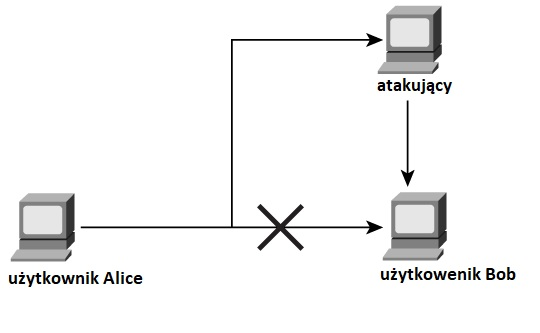
\includegraphics[width=7cm]{Powtarzajace_ataki.jpg}
\caption{Człowiek w środku - powtarzanie sesji}\label{Powtarzajace_ataki}
\end{figure}

\quad W atakach typu "porwanie sesji" atakujący dodaje się do połączenia między dwoma użytkownikami w celu przejęcia komunikacji między nimi. Na rysunku poniżej pokazano schematycznie atak typu "porwanie sesji". Użytkownik Alice wysyła wiadomość do użytkownika Bob, jednak na drodze odczytuje ją atakujący, który przez Alice jest traktowany jako użytkownik Bob. Następnie atakujący przesyła wiadomość do prawdziwego Boba i po otrzymaniu jego odpowiedzi przesyła ją do użytkownika Alice po zmodyfikowaniu. Atakujący dołącza się do połączeń w celu znalezienie luk z zabezpieczeniach. Na rys.~\ref{Porwanie_sesji} przedstawiono schemat ataku typu człowiek w środku - porwanie sesji.
\begin{figure}[H]
\centering
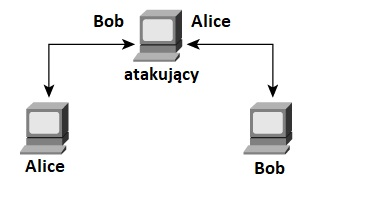
\includegraphics[width=8cm]{Porwanie_sesji.jpg}
\caption{Człowiek w środku - porwanie sesji}\label{Porwanie_sesji}
\end{figure}

\quad Prywatna wirtualna sieć zapewnia trzy etapy chroniące nas przed niepożądanymi atakami w wystarczający sposób. Pierwszym z nich jest uwierzytelnienie urządzenia, które chroni przed przechwytywaniem pakietów przez zamaskowane urządzenia atakujące. Następnym krokiem jest sprawdzenie integralności pakietów np. przy użyciu funkcji haszujących. Trzecim etapem jest zaszyfrowanie pakietów, co znacznie utrudnia przechwycenie rzeczywistych informacji.
\end{itemize}


\subsection{Maszyna Enigma}

\subsection{Szyfry blokowe i strumieniowe}
\subsubsection{Szyfry blokowe} 
\quad Szyfry blokowe wykorzystywane są do szyfrowania i deszyfrowania. Danymi wejściowymi do szyfrowania jest blok danych, który przy użyciu klucza szyfrującego jest przekształcany w zaszyfrowany blok danych. Odszyfrowywanie przebiega w odwrotny sposób, zaszyfrowana blokowa wiadomość przy użyciu klucza jest transformowana do odszyfrowanej blokowej wiadomości. Szyfr blokowy jest bezpieczny do momentu kiedy klucz szyfrujący pozostaje tajny. Bez znajomości klucza niemożliwe staje się rozszyfrowanie wiadomości w satysfakcjonującym nas czasie. Im bardziej klucz jest przypadkowy tym ciężej złamać algorytm. Ważnymi parametrami szyfru blokowego jest rozmiar bloku i klucza od których to zależy bezpieczeństwo algorytmu. Powszechnie stosowanymi rozmiarami bloków są 64 i 128 bitowe bloki, zazwyczaj algorytm DES ma 64 bitowy blok danych, zaś AES 128 bitowy blok. W tabeli~\ref{bajt} ukazano, że rozmiar 1 bajta odpowiada rozmiarowi 8 bitów.
\begin{table}[H]
\centering
\begin{tabular}{|r|r|r|c|c|l|l|l|}
\hline
1 bit & 1 bit & 1 bit & 1 bit & 1 bit & 1 bit & 1 bit & 1 bit\\
\hline
\multicolumn{8}{|c|}{1 bajt = 8 bitów}\\
\hline
\end{tabular}
\caption{Rozmiar jednego bajta.}\label{bajt}
\end{table}

\quad Długość zaszyfrowanego bloku musi być optymalna, im większe bloki danych tym dłuższy zaszyfrowany tekst oraz użycie pamięci. Przy szyfrowaniu wiadomości która na długość 8 bitową, zaś blok szyfru ma długość 64 bity najpierw 8 bitowa wiadomość zostanie prze konwertowana na 64 bitowy blok. Następnie 64 bitowa wiadomość zostanie zaszyfrowana przy użyciu algorytmu tworząc zaszyfrowany tekst. Do przetworzenia szyfru blokowego o rozmiarze 64 bitów potrzebujemy 64 bitów pamięci w rejestrach procesora. W dzisiejszych czasach procesory z pamięcią 64 bitową nie są kosztowne, lecz im większy chcemy utworzyć blok szyfrowy tym lepszy procesor potrzebujemy, co może mieć znaczny wpływ na wysokie koszty.

\subsubsection{Szyfry strumieniowe}
\quad Szyfrowanie strumieniowe jest deterministyczne, co oznacza, że przy jednakowych danych wejściowych otrzymujemy taki sam wynik wyjściowy. Dzięki determinizmowi możliwe jest odszyfrowanie zaszyfrowanych strumieni bitów.  Szyfrowanie strumieniowe jest podobne w działaniu do deterministycznego generatora liczb pseudolosowych, z tą różnicą że szyfrowanie strumieniowe oprócz wartości wejściowej pobiera dodatkowo klucz, który zazwyczaj ma 128 lub 256 bitów długości. Strumieniem klucza jest pseudolosowym strumieniem bitów. Szyfrowanie strumieniowe polega na przekształceniu tekstu jawnego bit po bicie na szyfrogram. Elementy tworzące szyfrowanie strumieniowe to generator strumienia bitowy oraz element dodający np. operacja XOR. Operację XOR-owania przedstawiono w tabeli~\ref{xor}.

\begin{table}[H]
\centering
\begin{tabular}{|r|c|l|}
\hline
p & q & p $\veebar$ q \\
\hline
0 & 0 & \multicolumn{1}{|c|}{0} \\
\hline
0 & 1 & \multicolumn{1}{|c|}{1} \\
\hline
1 & 0 & \multicolumn{1}{|c|}{1} \\
\hline
1 & 1 & \multicolumn{1}{|c|}{0} \\
\hline
\end{tabular}
\caption{Tablica dla operacji XOR.}\label{xor}
\end{table}

Proces XOR-owania przebiega następująco:
\begin{itemize}
\item wiadomość jako tekst jawny \newline
\begin{center}
01001101
\end{center}
\item strumień klucza wytworzony przez generator strumienia klucza \newline
\begin{center}
00111000
\end{center}
\item XOR-owana wiadomość (szyfrogram) \newline
\begin{center}
01110101
\end{center}
\end{itemize}
Szyfrowanie strumieniowe polega na operacji xor tekstu jawnego(P) ze strumieniem klucza(KS) w wyniku czego otrzymano zaszyfrowaną wiadomość(C).\newline
\begin{center}
C = P $\oplus$ KS
\end{center}
Proces deszyfrowania strumieniowego polega na operacji xor tekstu zaszyfrowanego(C) z strumieniem klucza(KS), w wyniku czego otrzymano tekst jawny(P).~\cite{stream_cipher}\newline
\begin{center}
P = C $\oplus$ KS
\end{center}

\subsection{Szyfry symetryczne i asymetryczne}

\subsubsection{Szyfry symetryczne}
\quad Do szyfrów symetrycznych zaliczamy zarówno szyfry blokowe jak i strumieniowe. Szyfrowanie symetryczne używa jednego tajnego klucza do szyfrowania i odszyfrowywania wiadomości. W celu zaszyfrowania tekstu jawnego przy użyciu tajnego klucza szyfrujemy wiadomość do postaci tekstu zaszyfrowanego, co przedstawia rys.~\ref{szyfrowanie}.
\newline
\begin{figure}[H]
\begin{center}
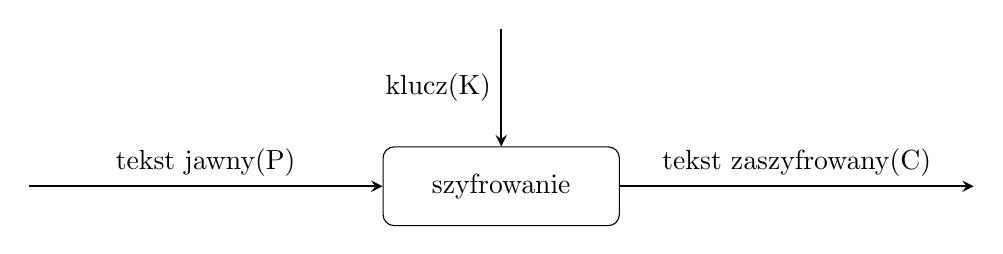
\begin{tikzpicture}
\node (start) [prostokat] {szyfrowanie};
\draw [arrow] (start) -- node[anchor=south] {tekst zaszyfrowany(C)} (6,0);
\draw [arrow] (-6,0) -- node[anchor=south] {tekst jawny(P)} (start);
\draw [arrow] (0,2) -- node[anchor=east] {klucz(K)} (start);
\end{tikzpicture}
\end{center}
\caption{Schematyczny proces szyfrowania symetrycznego.}\label{szyfrowanie}
\end{figure}

Proces odszyfrowywania polega na przekształceniu tekstu zaszyfrowanego przy użyciu klucza w tekst jawny. Klucz jest taki sam dla procesu szyfrowania i odszyfrowywania. Na rys.~\ref{odszyfrowanie} ukazano schematycznie proces odszyfrowywania symetrycznego.
\newline
\begin{figure}[H]
\begin{center}
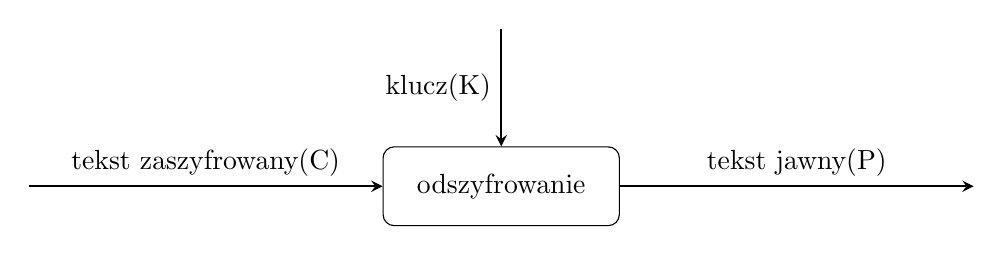
\begin{tikzpicture}
\node (start) [prostokat] {odszyfrowanie};
\draw [arrow] (start) -- node[anchor=south] {tekst jawny(P)} (6,0);
\draw [arrow] (-6,0) -- node[anchor=south] {tekst zaszyfrowany(C)} (start);
\draw [arrow] (0,2) -- node[anchor=east] {klucz(K)} (start);
\end{tikzpicture}
\end{center}
\caption{Schematyczny proces odszyfrowania symetrycznego.}\label{odszyfrowanie}
\end{figure}

Przed erą urządzeń obliczających używano szyfry klasyczne, które działały na literach, a nie na bitach. Do szyfrów klasycznych zaliczamy słynny szyfr Cezara.
\paragraph{szyfr Cezara}
\quad 

Szyfr Cezara zawdzięcza swoją nazwę Juliuszowi Cezarowi, który to już w czasach starożytnych był wykorzystywany przez Juliusza. Szyfr służył do szyfrowania wiadomości poprzez zastąpienie litery literą o 3 miejsca przesuniętą względem wartości początkowej np. literę A zastąpiono literą C. W tabeli~\ref{cezar} ukazano obrazowo podstawienie z przesunięciem o trzy litery.

\begin{table}[H]
\centering
\begin{tabular}{|c|c|c|c|c|c|c|c|c|c|c|c|c|c|c|c|c|c|}
\hline
podstawa & A & Ą & B & C & Ć & D & E & Ę & F & G & H & I & J & K & L & Ł & M \\
\hline 
\hline
podstawienie & C & Ć & D & E & Ę & F & G & H & I & J & K & L & Ł & M & N & Ń & O \\
\hline
\hline
podstawa & N & Ń & O & Ó & P & R & S & Ś & T & U & W & X & Y & Z & Ż & Ź & \\
\hline 
\hline
podstawienie & Ó & P & R & S & Ś & T & U & W & X & Y & Z & Ż & Ź & A & Ą & B & \\
\hline
\end{tabular}
\caption{Szyfr Cezara z przesunięciem o trzy litery.}~\label{cezar}
\end{table}

Szyfr ten nie zapewnia bezpieczeństwa, gdyż bez problemu i w krótkim czasie można przetestować wszystkie możliwe 33 opcje w przypadku języka polskiego. Szyfr ten uniemożliwia natychmiastowe zinterpretowanie wysyłanej wiadomości po jej ujrzeniu.

\paragraph{DES}\mbox{} \\

Algorytm zwany standardem szyfrowania danych (ang. Data Encryption Standard DES) został opatentowany przez firmę IBM i rozpowszechniony w latach siedemdziesiątych do ogólnego użytku, początkowo miał nazwę Lucyfer. We wczesnych latach siedemdziesiątych nie znane były nikomu algorytmy szyfrowania do momentu opatentowania przez firmę IBM algorytmu DES i jego rozpowszechnienia. Standard szyfrowania danych jest szyfrem blokowych, co znaczy że dane są dzielone na bloki o długości 64 bitów i następnie szyfrowane. Danymi wejściowymi algorytmu jest blok tekstu jawnego o długości 64 bitów, który po przetworzeniu przez algorytm przedstawiono jako szyfrogram. Długość klucza w 64 bitowym bloku wynosi 56 bitów, gdzie co ósmy bit jest bitem parzystości. Algorytm DES składa się z 16 cykli, które są wykonywane jeden po drugim. Na schemacie XXX poglądowo pokazano schemat działania algorytmu DES. Algorytm można podzielić na poszczególne kroki:

\begin{itemize}
\item zamiana 64 bitowego klucza decymalnego na postać binarną i usunięcie co ósmego bitu zwanego bitem parzystości w wyniku czego otrzymano 56 bitowy binarny klucz
\item permutacja 56 bitowego klucza binarnego zgodnie z tabelą~\ref{per_klucza} dla każdego z 16 cykli
\item podział 56 bitowego klucza na prawą o lewą część o długości 28 bitów i przesunięcie bitowe, które jest zależne od cyklu co ukazuje tabela~\ref{przesuniecie_klucza}
\item permutacja kompresji klucza DES zgodnie z tabelą~\ref{per_kompresji} kompresująca klucz 56 bitowy do klucza 48 bitowego dla każdego z 16 cykli ukazanego na rysunku~\ref{des} jako  K{i}
\item zamiana wiadomości tekstowej na wiadomość w postaci heksadecymalnej i binarną
\item transpozycja wiadomości binarnej z tabelą permutacji początkowej
\item podział wiadomości 64 bitowej na dwie części 32 bitowe: strona prawa oznaczona literą P na rysunku~\ref{des} i strona lewa oznaczona literą L na rysunku~\ref{des}
\item prawa cześć wiadomości ulega rozszerzeniu zgodnie z tabelą~\ref{per_rozszerzenia} permutacji rozszerzenia w wyniku czego otrzymano 48 bitową wiadomość
\item operacja XOR obliczonego klucza dla danej rundy z 48 bitową wiadomością otrzymaną w wyniku permutacji rozszerzenia
\item transpozycją wyniku operacji XOR z tablicą S bloków na rysunku~\ref{des} oznaczono S-boxes
\item wyjście S bloku ulega transpozycji z tabelą permutacji bloku P na rysunku~\ref{des} oznaczono jako P box
\item wiadomość po permutacji bloku P poddano operacji XOR z lewą częścią wiadomości w wyniku czego otrzymano 32 bitową część prawą wiadomości
\item lewą częścią 32 bitowej wiadomości jest prawa część 32 bitowej wiadomości bez żadnych zmian
\end{itemize}
Dane wyjściowe wiadomości z rundy pierwszej są danymi wejściowymi dla rundy drugiej algorytmu. Kroki przedstawione powyżej należy wykonać 16 razy w calu zaszyfrowania wiadomości, która jest podzielona na bloki 64 bitowe. Na obrazku~\ref{des} zobrazowano pojedynczą rundę algorytmu DES.

\begin{figure}[H]
\centering
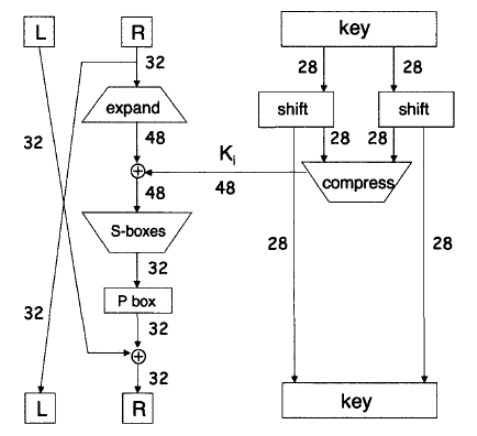
\includegraphics{des}
\caption{Pojedyncza runda algorytmu DES.~\cite{DES}
}\label{des}
\end{figure}

W tabeli~\ref{hex_to_bin} ukazano reprezentację binarną liczą heksadecymalnych w systemie 64 bitowym.

\begin{table}[H]
\centering
\begin{tabular}{|c|c|c|c|c|c|c|c|c|}
\hline
0 & 1 & 2 & 3 & 4 & 5 & 6 & 7\\
\hline
0000 & 0001 & 0010 & 0011 & 0100 & 0101 & 0110 & 0111\\
\hline
8 & 9 & A & B & C & D & E & F\\
\hline
1000 & 1001 & 1010 & 1011 & 1100 & 1101 & 1110 & 1111\\
\hline
\end{tabular}
\caption{Reprezentacja binarna liczb heksadecymalnych.}~\label{hex_to_bin}
\end{table}

W tabeli~\ref{per_poczatkowa} przedstawiono tablicę dla permutacji początkowej wiadomości dla algorytmu DES. Permutacji dokonuje się poprzez zamianę miejscami bitów zgodnie z tabelą permutacji otrzymując w wyniku przekształcone dane wejściowe.

\begin{table}[H]
\centering
\begin{tabular}{|c|c|c|c|c|c|c|c|c|c|c|c|c|c|c|c|}
\hline
58 & 50 & 42 & 34 & 26 & 18 & 10 & 2 & 60 & 52 & 44 & 36 & 28 & 20 & 12 & 4\\
\hline
62 & 54 & 46 & 38 & 30 & 22 & 14 & 6 & 64 & 56 & 48 & 40 & 32 & 24 & 16 & 8\\
\hline
57 & 49 & 41 & 33 & 25 & 17 & 9 & 1 & 59 & 51 & 43 & 35 & 27 & 19 & 11 & 3\\
\hline
61 & 53 & 45 & 37 & 29 & 21 & 13 & 5 & 63 & 55 & 47 & 39 & 31 & 23 & 15 & 7\\
\hline
\end{tabular}
\caption{Permutacja początkowa DES.}\label{per_poczatkowa}
\end{table}

Tabela~\ref{per_klucza} ukazuje permutacje klucza 56 bitowego, który powstaje z klucza 64 bitowego w wyniku usunięcia co ósmego bitu parzystości.%Czemu usuwamy bit parzystości?

\begin{table}[H]
\centering
\begin{tabular}{|c|c|c|c|c|c|c|c|c|c|c|c|c|c|}
\hline
57 & 49 & 41 & 33 & 25 & 17 & 9 & 1 & 58 & 50 & 42 & 34 & 26 & 18\\
\hline
10 & 2 & 59 & 51 & 43 & 35 & 27 & 19 & 11 & 3 & 60 & 52 & 44 & 36\\
\hline
63 & 55 & 47 & 39 & 31 & 23 & 15 & 7 & 62 & 54 & 46 & 38 & 30 & 22\\
\hline
14 & 6 & 61 & 53 & 45 & 37 & 29 & 21 & 13 & 5 & 28 & 20 & 12 & 4 \\
\hline
\end{tabular}
\caption{Permutacja klucza DES.}~\label{per_klucza}
\end{table}
 
Przesunięcia bitowe dwóch kluczy 28 bitowych tworzących wejściowy klucz 56 bitowy dla każdego cyklu zależą od numeru cyklu, co ukazano w tabeli~\ref{przesuniecie_klucza}.

\begin{table}[H]
\begin{tabular}{|c|c|c|c|c|c|c|c|c|c|c|c|c|c|c|c|c|}
\hline
cykl&1&2&3&4&5&6&7&8&9&10&11&12&13&14&15&16\\
\hline
liczba przesunięć&1&1&2&2&2&2&2&2&1&2&2&2&2&2&2&1\\ \hline
\end{tabular}
\caption{Liczba przesunięć klucza w zależności od cyklu.}\label{przesuniecie_klucza}
\end{table} 
 
Po operacji przesunięcia bitowego klucza 56 bitowego wykonano kompresję klucza do rozmiaru 48 bitów zgodnie z tabelą~\ref{per_kompresji}.
 
\begin{table}[H]
\centering
\begin{tabular}{|c|c|c|c|c|c|c|c|c|c|c|c|}
\hline
14 & 17 & 11 & 24 & 1 & 5 & 3 & 28 & 15 & 6 & 21 & 10\\
\hline
23 & 19 & 12 & 4 & 26 & 8 & 16 & 7 & 27 & 20 & 13 & 2\\
\hline
41 & 52 & 31 & 37 & 47 & 55 & 30 & 40 & 51 & 45 & 33 & 48\\
\hline
44 & 49 & 39 & 56 & 34 & 53 & 46 & 42 & 50 & 36 & 29 & 32\\
\hline
\end{tabular}
\caption{Permutacja kompresji DES.}~\label{per_kompresji}
\end{table}

Tabela~\ref{per_rozszerzenia} jest stosowana do operacji rozszerzenia wiadomości. Wiadomość 64 bitowa zostaje podzielona na dwa 32 bitowe bloki, które następnie ulegają rozszerzeniu do dwóch 48 bitowych bloków zgodnie z tabelą~\ref{per_rozszerzenia} permutacji rozszerzenia. Rozszerzone 48 bitowe bloki zawierają powtórzenia bitów, rozszerzenie 32 do 48 bitów powoduję wystąpienie 16 bitów które nie są unikatowe. Oznacza to, że 8 bitów występuje podwójnie w szyfrowanej wiadomości.

\begin{table}[H]
\centering
\begin{tabular}{|c|c|c|c|c|c|c|c|c|c|c|c|}
\hline
32 & 1 & 2 & 3 & 4 & 5 & 4 & 5 & 6 & 7 & 8 & 9\\
\hline
8 & 9 & 10 & 11 & 12 & 13 & 12 & 13 & 14 & 15 & 16 & 17\\
\hline
16 & 17 & 18 & 19 & 20 & 21 & 20 & 21 & 22 & 23 & 24 & 25\\
\hline
24 & 25 & 26 & 27 & 28 & 29 & 28 & 29 & 30 & 31 & 32 & 1\\
\hline
\end{tabular}
\caption{Permutacja rozszerzenia DES.}~\label{per_rozszerzenia}
\end{table}

Po dokonaniu permutacji rozszerzenia wiadomości dokonano operacji xor otrzymanej wiadomości z obliczonym kluczem dla danego cyklu. Otrzymany wynik podzielono na 8 bloków 6 bitowych, które wykorzystano do dalszych obliczeń z pomocą tabeli~\ref{s_bloki} s bloków. Z każdego bloku 6 bitowego odczytano wartość pierwszego i ostatniego bitu, wartość 00 oznacza wykorzystanie wiersza pierwszego z danego bloku, 01 oznacza wiersz drugi, 10 oznacza wiersz trzeci, natomiast 11 oznacza wiersz czwarty. Wartości od bita drugiego do piątego zamieniamy na postać heksadecymalną i odczytujemy dla niej wartość z danego bloku np. jeśli pierwszy i ostatni bit to 00 to wartość odczytano z wiersza pierwszego, gdy bity między 2-5 pozycją to 1111 oznacza to ostatnią wartość z wiersza pierwszego czyli 7.

\begin{table}[H]
\centering
\begin{tabular}{|c|c|c|c|c|c|c|c|c|c|c|c|c|c|c|c|c|}
\hline
\multicolumn{16}{|c|}{S blok 1}\\ 
\hline
14&4&13&1&2&15&11&8&3&10&6&12&5&9&0&7 \\ \hline
0 &	15& 	7 &	4 &	14 &	2& 	13& 	1 &	10 &	6 &	12 &	11 &	9 &	5 &	3 &	8 \\ \hline
4 &	1 &	14 &	8 	&13 	&6 &	2& 	11& 	15& 	12 &	9 	&7& 	3& 	10& 	5& 	0 \\ \hline
15 &	12& 	8 &	2 &	4 &	9 &	1 &	7 &	5 &	11 &	3 &	14 &	10 &	0 &	6 &	13 \\ \hline
\multicolumn{16}{|c|}{S blok 2} \\ \hline
15 &	1 &	8 &	14 &	6 &	11 &	3 &	4 &	9 &	7 &	2 &	13 &	12 &	0 &	5 &	10 \\ \hline
3 &	13& 	4 &	7 &	15 &	2 &	8 &	14 &	12 &	0 &	1 &	10 &	6 &	9 &	11 &	5 \\ \hline
0 &	14 &	7 &	11 &	10 &	4 &	13 &	1 &	5 &	8 &	12 &	6 &	9 &	3 &	2 &	15 \\ \hline
13 &	8 &	10 &	1 &	3 &	15 &	4 &	2 &	11 &	6 &	7 &	12 &	0 &	5 &	14 &	9 \\ \hline
\multicolumn{16}{|c|}{S blok 3}\\ \hline
10 &	0 &	9 &	14 &	6 &	3 &	15 &	5 &	1 &	13 &	12 &	7 &	11 &	4 &	2 &	8\\ \hline
13 &	7 &	0 &	9 &	3 &	4 &	6 &	10 &	2 &	8 &	5 &	14 &	12 &	11 &	15 &	1\\ \hline
13 &	6 &	4 &	9 &	8 &	15 &	3 &	0 &	11 &	1 &	2 &	12 &	5 &	10 &	14 &	7\\ \hline
1 &	10 &	13 &	0 &	6 &	9 &	8 &	7 &	4 &	15 &	14 &	3 &	11 &	5 &	2 &	12 \\ \hline
\multicolumn{16}{|c|}{S blok 4}\\ \hline
7 &	13 &	14 &	3 &	0 &	6 &	9 &	10 &	1 &	2& 	8& 	5& 	11& 	12& 	4& 	15\\ \hline
13& 	8& 	11& 	5& 	6& 	15& 	0& 	3& 	4& 	7& 	2& 	12& 	1& 	10& 	14& 	9\\ \hline
10& 	6& 	9& 	0& 	12& 	11& 	7& 	13& 	15& 	1& 	3& 	14& 	5& 	2& 	8& 	4\\ \hline
3& 	15& 	0& 	6& 	10& 	1& 	13& 	8& 	9& 	4& 	5& 	11& 	12& 	7& 	2& 	14\\ \hline
\multicolumn{16}{|c|}{S blok 5}\\ \hline
2& 	12& 	4& 	1& 	7& 	10& 	11& 	6& 	8& 	5& 	3& 	15& 	13& 	0& 	14& 	9\\ \hline
14& 	11& 	2& 	12& 	4& 	7& 	13& 	1& 	5& 	0& 	15& 	10& 	3& 	9& 	8& 	6\\ \hline
4& 	2& 	1& 	11& 	10& 	13& 	7& 	8& 	15& 	9& 	12& 	5& 	6& 	3& 	0& 	14\\ \hline
11& 	8& 	12& 	7& 	1& 	14& 	2& 	13& 	6& 	15& 	0& 	9& 	10& 	4& 	5& 	3\\ \hline 
\multicolumn{16}{|c|}{S blok 6}\\ \hline
12& 	1& 	10& 	15& 	9& 	2& 	6& 	8& 	0& 	13& 	3& 	4& 	14& 	7& 	5& 	11\\ \hline
10 &	15& 	4& 	2& 	7& 	12& 	9& 	5& 	6& 	1& 	13& 	14& 	0& 	11& 	3& 	8\\ \hline
9& 	14& 	15& 	5& 	2& 	8& 	12& 	3& 	7& 	0& 	4& 	10& 	1& 	13& 	11& 	6\\ \hline
4& 	3& 	2& 	12& 	9& 	5& 	15& 	10& 	11& 	14& 	1& 	7& 	6& 	0& 	8& 	13\\ \hline
\multicolumn{16}{|c|}{S blok 7}\\ \hline
4& 	11& 	2& 	14& 	15& 	0& 	8& 	13& 	3& 	12& 	9& 	7& 	5& 	10& 	6& 	1\\ \hline
13& 	0& 	11& 	7& 	4& 	9& 	1& 	10& 	14& 	3& 	5& 	12& 	2& 	15& 	8& 	6\\ \hline
1& 	4& 	11& 	13& 	12& 	3& 	7& 	14& 	10& 	15& 	6& 	8& 	0& 	5& 	9& 	2\\ \hline
6& 	11& 	13& 	8& 	1& 	4& 	10& 	7& 	9& 	5& 	0& 	15& 	14& 	2& 	3& 	12\\ \hline 
\multicolumn{16}{|c|}{S blok 8}\\ \hline
13& 	2& 	8& 	4& 	6& 	15& 	11& 	1& 	10& 	9& 	3& 	14& 	5& 	0& 	12& 	7\\ \hline
1& 	15& 	13& 	8& 	10& 	3& 	7& 	4& 	12& 	5& 	6& 	11& 	0& 	14& 	9& 	2\\ \hline
7& 	11& 	4& 	1& 	9& 	12& 	14& 	2& 	0& 	6& 	10& 	13& 	15& 	3& 	5& 	8\\ \hline
2& 	1& 	14& 	7& 	4& 	10& 	8& 	13& 	15& 	12& 	9& 	0& 	3& 	5& 	6& 	11 \\ \hline
\end{tabular}
\caption{Struktury S bloków.}\label{s_bloki}
\end{table}



\begin{table}[H]
\centering
\begin{tabular}{|c|c|c|c|c|c|c|c|c|}
\hline
16 &	7 &	20& 	21& 	29& 	12& 	28& 	17\\ \hline
1 &	15& 	23& 	26& 	5& 	18& 	31& 	10\\ \hline
2 &	8 &	24 &	14& 	32& 	27& 	3 &	9\\ \hline
19 	&13 &	30& 	6& 	22& 	11& 	4& 	25\\ \hline
\end{tabular}
\caption{Permutacja bloku P.}~\label{blok_P}
\end{table}

Algorytm DES nie jest obecnie uznawany za bezpieczny przez Amerykańskie Standardy Federalne. W roku 2015 przy użyciu wysokiej wydajności FPGA możliwe było złamanie szyfru w stosunkowo krótkim czasie(4-5 dni). Dla atakujących przestała być odstraszająca cena platformy FPGA w porównaniu do zysków jakie może dać im atak. W celu przesłania klucza do drugiej osoby, z którą tworzymy bezpieczne połączenie wymaga znalezienie bezpiecznej metody przesyłu klucza. Zaletami algorytmu DES jest jego odporność na błędy, dzięki jego prostocie aplikacji. W obecnych czasach jest on nadal popularny w użytku, dzięki swojej szybkości.~\cite{DES}

%%% cos o deszyfracji dodac

\paragraph{AES} \mbox{} \\


\paragraph{IDEA} \mbox{} \\ 

IDEA to Międzynarodowy Algorytm Szyfrowania Danych(z ang. International Data Encryption Algorithm). Początkowo nosił nazwę PES(z ang. Proposed Encryption Standard) opatentowany przez Xuejia Lai i Jamesa Massey w 1990 roku. Następnie został on ulepszony przed atakiem zmieniając nazwę na IPES(z ang.Improved Proposed Encryption Standard). Ostatecznie jego nazwę zmieniono na obecnie używaną IDEA w 1992 roku. Jest to algorytm blokowy, który wykorzystuje bloki 64 bitowe i klucz o długości 128 bitów. Do szyfrowania i odszyfrowywania wykorzystuje się ten sam algorytm. Algorytm ten początkowo dzieli blok 64 bitowy na 4 pod bloki 16 bitowe, na których dokonywane są operację: XOR, dodawanie modulo i mnożenie modulo. Algorytm składa się z ośmiu rund. Na rysunku~\ref{idea} przedstawiono pojedyncza rundę algorytmu IDEA, gdzie pierwsza 16 bitowa część wiadomości podlega operacji mnożenia modulo z 16 bitowym kluczem rundy. Operacja modulo oznaczona przy pomocy kółka z kropką w środku $\odot$. Druga 16 bitowa część wiadomości poddano operacji dodawania modulo z 16 bitowym kluczem rundy. Operacje dodawania modulo oznaczono kwadratem z plusem w środku $\boxplus$. Operację XOR oznaczono okręgiem z plusem w środku $\oplus$. Operacje mnożenia, dodawania i xorowania są wykonywane na częściach wiadomości zgodnie z rysunkiem~\ref{idea}. Po operacjach xorowania, dodawania i mnożenia dokonujemy przestawienia bloku drugiego z trzecim, które są danymi wejściowymi do następnej rundy. W każdej rundzie używany jest 16 bitowy klucz dla danego pod bloku. Po zakończeniu ośmiu rund, cztery bloki są złożone do jednego bloku 64 bitowego, który jest wynikiem końcowym.

\begin{figure}[H]
\centering
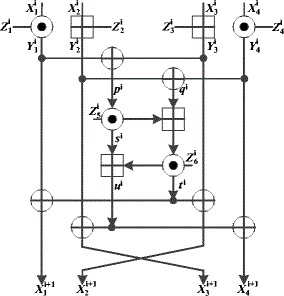
\includegraphics{IDEA.jpg}
\caption{Pojedyncza runda algorytmu IDEA.~\cite{IDEA}}\label{idea}
\end{figure}


Dla operacji dodawania modulo potrzebne są dwie liczby, na których zostanie wykonane działanie oraz tzn. licza modulo. Operacja dodawania modulo przebiega w następujących krokach: dodanie do siebie dwóch liczb, a następnie podzielenie wyniku dodawania przez liczbę modulo. Reszta z wyniku dzielenia sumy dwóch licz przez liczbę module daje nam wynik operacji dodawania modulo. Operacje dodawania modulo oznaczono symbolem $\boxplus$. Przykładem operacji dodawania modulo jest: 2 $\boxplus$ 5 $\equiv$ 1 (mod 3). Dla operacji mnożenia modulo potrzebne są dwie liczby, na których zostanie wykonane działanie oraz tzn. liczba modulo. Operacja mnożenia modulo polega na iloczynie dwóch czynników oraz ilorazie wyniku operacji z liczbą modulo. Wynikiem jest reszta z operaji dzielenia przez liczbę modulo.  Operacje mnożenia modulo oznaczono symbolem $\odot$. Przykładem operacji mnożenia modulo jest 2  $\odot$ 7 = 2 (mod 3), bo 2*7 = 14, gdzie 14/3 daje resztę z dzielenia 2.
Klucz o długości 128 bitów jest dzielony na osiem 16 bitowych podkluczy. Dla każdej rundy zostaje wykorzystane 6 podkluczy, które oznaczono na rysunku~\ref{idea} literą Z. Do wszystkich rund, których jest 8 użyto 52 podkluczy oraz 4 podklucze użyte do końcowych przekształceń. Dla algorytmu IDEA użyto łącznie 52 podkluczy, które stworzono z 128 bitowego klucza. Generację klucza 128 bitowego do 52 podkluczy można podzielić na:
\begin{itemize}
\item podział 128 bitowego klucza na 8 podkluczy 16 bitowych, gdzie pierwsze 6 podkluczy wykorzystano do rundy 1, a następne 2 podklucze użyto do rundy 2 algorytmu
\item przesunięcie klucza 128 bitowego w lewo o 25 bitów i ponowny podział na 8 podkluczy, gdzie pierwsze 4 podklucze użyto do rundy drugiej, a następne 4 podklucze wykorzystano w rundzie 3
\item klucz jest dalej analogicznie przesuwany i dzielony, aż do momentu uzyskania 52 podkluczy
\end{itemize}

Proces deszyfrowania wiadomości również korzysta z schematu przedstawionego na rysunku~\ref{idea} pojedynczej rundy algorytmu, składa się on również z 8 rund. Proces tworzenia podkluczy z klucza odbywa się na podstawie podkluczy wykorzystanych do zaszyfrowania wiadomości. Przy utworzeniu klucza pomocna jest tabela multiplikatywnej odwrotności 4 bitowej liczby binarnej przedstawionej w tabeli~\ref{nibel}.

\begin{table}[H]
\centering
\begin{tabular}{|c|c|c|}
\hline
\thead{wartość \\ binarna[decymalna]} & \thead{multiplikatywna \\  odwrotność[decymalna]} & \thead{addytywna \\ odwrotność[decymalna]}\\ \hline
0000 [0]&0000 [0]&0000 [0] \\ \hline
 0001 [1]&1111 [15]&0001 [1]\\ \hline
 0010 [2]&1110 [14]&1001 [9]\\ \hline
 0011 [3]&1101 [13]&0110 [6]\\ \hline
 0100 [4]&1100 [12]&1101 [13]\\ \hline
 0101 [5]&1011 [11]&0111 [7]\\ \hline
 0110 [6]&1010 [10]&0011 [3]\\ \hline
 0111 [7]&1001 [9]&0101 [5]\\ \hline
 1000 [8]&1000 [8]&1111 [15]\\ \hline
 1001 [9]&0111 [7]&0010 [2]\\ \hline
 1010 [10]&0110 [6]&1100 [12]\\ \hline
 1011 [11]&0101 [5]&1110 [14]\\ \hline
 1100 [12]&0100 [4]&1010 [10]\\ \hline
 1101 [13]&0011 [3]&0100 [4]\\ \hline
 1110 [14]&0010 [2]&1011 [11]\\ \hline
 1111 [15]&0001 [1]&1000 [8]\\ \hline
 \end{tabular}
\caption{Obliczenia multiplikatywnej i addytywnej odwrotności.~\cite{IDEAA}}\label{nibel}
\end{table}

Multiplikatywną odwrotność dla a wyliczono według zależności x mod n, gdzie a $\in$ $Z_{n}$ oraz n jest rozmiarem grupy. Do obliczenia odwrotności addytywnej wykorzystano rozszerzony algorytm Euklidesa, który oblicza liczby całkowite x i y wykorzystując zależność ax + ny = 1, gdzie a $\in$ $Z_{n}$. Proces tworzenia podkluczy wykorzystanych do deszyfrowania ukazano w tabeli~\ref{podklucze_deszyfrowania_idea}. Potęga oznaczona literą a określa multiplikatywną odwrotność danej liczby, potęga oznaczona jako m określa addytywną odwrotność podanej liczby.
% opisac addytywna odwrotnosc i dlaczego 0


\begin{table}[H]
\centering
\begin{tabular}{|c|c|c|c|c|c|c|c|c|c|c|c|c|}
\hline
cykl & \multicolumn{6}{|c|}{podklucze szyfrujące}  & \multicolumn{6}{|c|}{podklucze deszyfrujące} \\ \hline
1&$x_{1}$&$x_{2}$&$x_{3}$&$x_{4}$&$x_{5}$&$x_{6}$&$x_{49}^{a}$&$x_{50}^{m}$&$x_{51}^{m}$&$x_{52}^{a}$&$x_{47}$&$x_{48}$\\ \hline
2&$x_{7}$&$x_{8}$&$x_{9}$&$x_{10}$&$x_{11}$& $x_{12}$&$x_{43}^{a}$&$x_{45}^{m}$&$x_{44}^{m}$&$x_{46}^{a}$&$x_{41}$&$x_{42}$\\ \hline
3&$x_{13}$&$x_{14}$&$x_{15}$&$x_{16}$&$x_{17}$&$x_{18}$&$x_{37}^{a}$&$x_{39}^{m}$&$x_{38}^{m}$&$x_{40}^{a}$&$x_{35}$&$x_{36}$\\ \hline
4&$x_{19}$&$x_{20}$&$x_{21}$&$x_{22}$&$x_{23}$&$x_{24}$&$x_{31}^{a}$&$x_{33}^{m}$&$x_{32}^{m}$&$x_{34}^{a}$&$x_{29}$&$x_{30}$\\ \hline
5&$x_{25}$&$x_{26}$&$x_{27}$&$x_{28}$&$x_{29}$&$x_{30}$&$x_{25}^{a}$&$x_{27}^{m}$&$x_{26}^{m}$&$x_{28}^{a}$&$x_{23}$&$x_{24}$\\ \hline
6&$x_{31}$&$x_{32}$&$x_{33}$&$x_{34}$&$x_{35}$&$x_{36}$&$x_{19}^{a}$&$x_{21}^{m}$&$x_{20}^{m}$&$x_{22}^{a}$&$x_{17}$&$x_{18}$\\ \hline
7&$x_{37}$&$x_{38}$&$x_{39}$&$x_{40}$&$x_{41}$&$x_{42}$&$x_{13}^{a}$&$x_{15}^{m}$&$x_{14}^{m}$&$x_{16}^{a}$&$x_{11}$&$x_{12}$\\ \hline
8&$x_{43}$&$x_{44}$&$x_{45}$&$x_{46}$&$x_{47}$&$x_{48}$&$x_{7}^{a}$&$x_{9}^{m}$&$x_{8}^{m}$&$x_{10}^{a}$&$x_{5}$&$x_{6}$\\ \hline
dodatkowe 4 podklucze&$x_{49}$&$x_{50}$&$x_{51}$&$x_{52}$&&&$x_{1}^{a}$&$x_{2}^{m}$&$x_{3}^{m}$&$x_{4}^{a}$&&\\ \hline
\end{tabular}
\caption{Podklucze szyfrujące i deszyfrujące IDEA.}\label{podklucze_deszyfrowania_idea}
\end{table}

Jedną z podstawowych zalet algorytmu są proste operacje na bitach tj. mnożenie i dodawanie modulo oraz xorowanie. Do szyfrowania i deszyfrowania wiadomości wykorzystuje ten sam proces, natomiast podklucze są różne dla szyfrowania i odszyfrowywania. Algorytm IDEA wolniej szyfruje dane niż algorytm DES, jednak dzięki temu, że jego klucz jest dwa razy dłuższy niż w DES ataki brutalne są mniej skuteczne.~\cite{IDEA}
\paragraph{Blowfish} \mbox{} \\


\subsubsection{Szyfry asymetryczne}

\quad Szyfry asymetryczne charakteryzują się tym, że posiadają osobny klucz do szyfrowania i osobny deszyfrowania. W celu wyjaśnienia zasady działania szyfru asymetrycznego przedstawiono powszechnie znany sposób wysyłania wiadomości od Alicji do Boba. Do szyfrowania używany jest klucz publiczny, natomiast do odszyfrowania wiadomości użyto klucza prywatnego. Bob generuje publiczny klucz, który może być znany dla każdego, gdyż tylko Bob mający klucz prywatny może odszyfrować wiadomość zaszyfrowaną przy pomocy jego publicznego klucza. Szyfrowanie asymetryczne jest bezpieczne nawet w przypadku wystąpienia osoby trzeciej Ewy, która chciałaby podsłuchać konwersację między Bobem, a Alicją. Bob po wygenerowaniu klucza publicznego wysyła go do Alicji, aby ta mogą zaszyfrować wiadomość, którą chce do niego przesłać. W przypadku gdy Ewa przechwyci klucz publiczny Boba, nie jest w stanie odszyfrować wiadomości, gdyż nie posiada klucza prywatnego Boba, w którego posiadaniu jest tylko on. W celu przesłania wiadomości od Boba do Alicji proces wygląda tak samo. Alicja generuje klucz publiczny, który wysyła do Boba. Bob szyfruje wiadomość publicznym kluczem Alicji i przesyła jej zaszyfrowaną wiadomość, która Alicja odszyfruje przy użyciu jej klucza prywatnego. Obecność dwóch kluczy w algorytmie rozwiązuje problem wymiany klucza, co pozwala osobom będącym daleko od siebie w bezpieczny sposób się komunikować.  







\begin{figure}[H]
\begin{center}
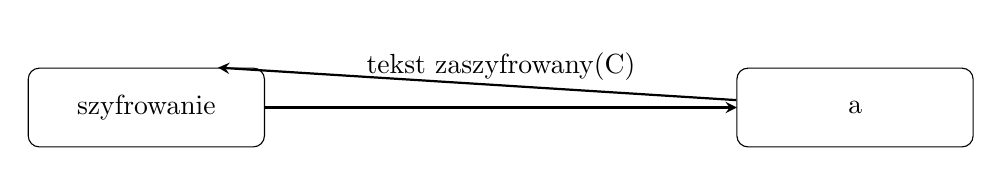
\begin{tikzpicture}
\node (ss) [prostokat] {szyfrowanie};
\draw [arrow] (ss)[prostokat] -- node[anchor=south] {tekst zaszyfrowany(C)} (7.5,0);
\node [prostokat,xshift=9cm] (a) {a};
\draw [arrow] ([yshift=5cm]a) -- (ss);

\end{tikzpicture}
\end{center}
\caption{Schematyczny proces szyfrowania asymetrycznego.}\label{szyfrowanie}
\end{figure}

\paragraph{RSA} \mbox{} \\

Algorytm RSA jest jednym z powszechniejszym algorytmów. Algorytm RSA zawdzięcza swoją nazwę trzem osobom, przez które został on opatentowany przez Rona Rivest, Adi Shamir i Leonard Adleman w 1977 roku. Nazwa algorytmu RSA pochodzi od pierwszych liter nazwisk wynalazców. Algorytm RSA bazuje na liczbach pierwszych oraz faktoryzacji dużych liczb. Proces tworzenia pary kluczy: prywatnego i publicznego przebiega w następujących krokach:
\begin{itemize}
\item wybór dwóch odpowiednio dużych licz pierwszych, które po przemnożeniu dadzą klucz o pożądanym rozmiarze np. 2048 bitów
\begin{center}
n = p * q 
\end{center}
,gdzie n = wynik mnożenia liczb pierwszych, p i q liczby pierwsze.
\item obliczenie funkcji Eulera według zależności
\begin{center}
m = (p-1)(q-1)
\end{center}
\item określenie liczby e względnie pierwszej z m oraz spełnia zależność 1<e<m
\item obliczenie liczby d według zależności
\begin{center}
d*e mod(m) = 1
\end{center}
\item obliczone liczby e i d są publiczne, natomiast liczba d jest trzymana w tajemnicy
\item zaszyfrowanie wiadomości c z wykorzystaniem wartości publicznych
\begin{center}
c = $m^{e}$mod(n)
\end{center}
\item do odszyfrowania wiadomości wykorzystano liczbę prywatną d według zależności
\begin{center}
p = $c^{d}$mod(n)
\end{center}
\end{itemize}
 
 
 
\paragraph{Diffie-Hellman} \mbox{} \\

Algorytm Diffie-Hellman został opatentowany w 1976 roku przez Whitfield Diffie i Martin Hellman. Dzięki temu algorytmowi możliwe jest przesyłanie klucza przez niezabezpieczone łącze w bezpieczny sposób. Obecnie jest on stosowany do wymiany klucza symetrycznego. Algorytm można opisać w następujących krokach: 
\begin{itemize}
\item Alicja generuje prywatną liczbę całkowitą a
\item Bob generuje prywatną liczbę całkowitą b
\item wybór liczby pierwszej p
\item obliczenie publicznej wartości z wykorzystaniem liczby piwerszej p, wartości g oraz prywatnej liczby a (dla Alicji) i b (dla Boba) według zależności
\begin{center}
$g^{a}$mod(p) i $g^{b}$mod(p)
\end{center}
\item wymiana publicznej wartości między Alicją i Bobem
\item Alicja oblicza
\begin{center}
$g^{ab}$ = $(g^{b})^{a}$mod(p)
\end{center}
\item Bob oblicza
\begin{center}
$g^{ba}$ = $(g^{a})^{b}$mod(p)
\end{center}
\item Alicja i Bob posiadają wspólny tajny klucz k, gdyż
\begin{center}
$g^{ab}$ = $g^{ba}$
\end{center}
\end{itemize}

Algorytm Diffie-Hellmana przestanie być bezpieczny w momencie, gdy zostanie rozwiązany problem logarytmu dyskretnego. Wartościami publicznymi powiązanymi poniższą relacją są g, p, a i b.
\begin{center}
$g^{a}$ $\equiv$ a mod(p) oraz $g^{b}$ $\equiv$ b mod(p)
\end{center}
Obecnie nie istnieje żaden algorytm umożliwiający rozwiązanie problemu logarytmu dyskretnego.~\cite{DH}

\paragraph{Funkcje haszujące} \mbox{} \\

\subsection{Protokoły}
\subsubsection{VPN with Point-to-Point Tunneling Protocol (PPTP)}
\quad Protokół punkt - punt często wykorzystywany na urządzeniach z systemem operacyjnym Windows w celu utworzenia wirtualnej sieci prywatnej. Protokół PPTP został utworzony w czasach sieci wdzwanianej tzn. dial up, jednak bez problemu można z niego korzystać również dla sieci Ethernet, Internet czy cyfrowa sieć usług zintegrowanych(ISDN). Utworzenie sicei VPN w sieci TCP/IP umożliwia bezpieczny transfer danych między zdalnym komputerem, a serwerem. Do implementacji protokołu głównie jest wykorzystywany: klient PPTP, serwer NAS i serwer PPTP. Serwer NAS bezpiecznie przechowuje dane i udostępnia je tylko wybranym użytkownikom. Na rys.~\ref{PPTP} poniżej poglądowo przedstawiono komunikację z użyciem protokołu PPTP. 
\begin{figure}[H]
\centering
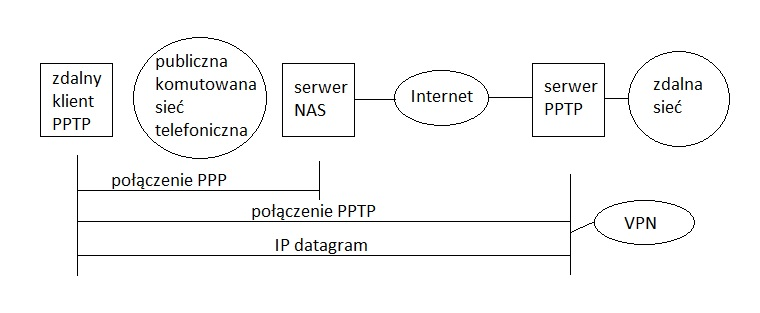
\includegraphics[width=12cm]{komunikacja_PPTP.jpg}
\caption{Poglądowa komunikacja z użyciem protokołu PPTP}\label{PPTP}
\end{figure}

Połączenie między zdalnym klientem, a siecią przebiega w określonych etapach:
\begin{itemize}
\item nawiązanie połączenia z użyciem protokołu komunikacyjnego point-to-point (PPP) między dwoma węzłami sieci w sposób telefoniczny bądź przewodowy z Internetem
\item połączenie PPP z serwerem PPTP, co tworzy połączenie VPN między zdalnym klientem, a serwerem
\end{itemize}
Po ustanowieniu połączenia wysyłane są dwa pakiety danych: pakiet kontrolny, który zarządza tunelem i pakiet danych. Protokół PPTP jest zaaplikowany na drugim poziomie modelu odniesienia łączenia systemów otwartych (OSI), który jest warstwą łącza danych. Jego działanie jest oparte na protokole punkt-punkt (PPP), który umożliwia korzystanie z usług internetowych. Protokół PPTP umożliwia firmom tworzenie prywatnych tuneli w publicznym internecie. Organizacje nie muszą już instalować kosztownych linii do komunikacji, dzięki protokołowi PPTP mogą w bezpieczny sposób korzystać z sieci publicznej w celu przesyłania poufnych danych. Protokół PPTP wspiera szyfrowanie i kompresję danych. Protokół PPTP nie jest wykorzystywany powszechnie ze względu na podatność na ataki.~\cite{PPTP}
\subsubsection{Secure Shell (SSH)}
\quad SSH z angielskiego to Secure Shell, co znaczy bezpieczna powłoka. Protokół SSH został wprowadzony w celu ulepszenia istniejących już wcześniej protokołów takich jak telnet, ftp czy BSD r-commands(rlogin, rexec, rsh,rcp). Protokoły telnet, ftp czy rsh były wykorzystywane do transferu plików między hostem lokalnym i zdalnym. Wymienione protokoły nadal są w powszechnym użytku, tylko tam gdzie bezpieczeństwo nie jest istotnym czynnikiem. Istotną wadą usług telnet i ftp jest brak szyfrowania i uwierzytelniania podczas przesyłania pakietów. Dane wysyłane są w sposób jawny, które mogą być w łatwiejszy sposób przechwycone przez atakującego. Atakujący może uzyskać niezaszyfrowane hasło, które następnie może wykorzystać w łatwy sposób. Wszędzie tam gdzie bezpieczeństwo danych jest ważne stosujemy protokół SSH. 
\quad SSH jest protokołem warstwy transportowej, która używa TCP do przenoszenia swoich pakietów. TCP jest protokołem sterowanie transmisją między dwoma urządzeniami. SSH umożliwia bezpieczne tunelowanie między lokalnym z zdalnym urządzeniem. Na poniższym rysunku przedstawiono komunikacje lokalnego klienta z powłoką serwera przy pomocy przekierowaniu portów. Na rys.~\ref{SSH} ukazano schemat lokalnego przekierowania portu dla protokołu SSH.
\begin{figure}[H]
\centering
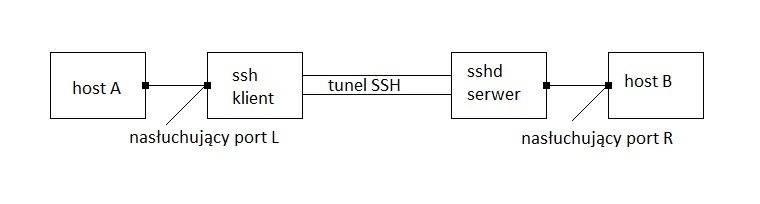
\includegraphics[width=12cm]{przekierowywanie_lokalne_SSH.jpg}
\caption{SSH lokalne przekierowywanie portu}\label{SSH}
\end{figure}

Host A wykonuje bezpiecznie połączenie do hostu B poprzez port R. Połączenie hostu A z hostem B przebiega w następujący sposób:
\begin{itemize}
\item host A łączy się do porty L na kliencie SSH
\item SSH przekierowuje połączenie poprzez bezpieczny tunel do serwera SSH
\item serwer SSH łączy się z hostem B poprzez port R
\end{itemize}
\newpage Port L na hoście A i port R na hoście B ustawione są w trybie ciągłego nasłuchiwania dla lokalnego połączenia. Na rys.~\ref{SSH_1} przedstawiono zdalne przekierowywanie portu z hosta B do hosta.
 
\begin{figure}[H]
\centering
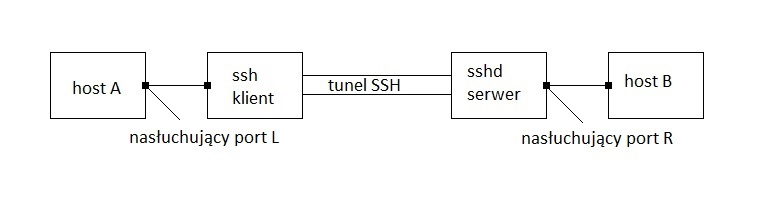
\includegraphics[width=10cm]{przekierowywanie_zdalne_SSH.jpg}
\caption{SSH zdalne przekierowywanie portu}\label{SSH_1}
\end{figure}

Zdalne przekierowanie portu przebiega w następujących krokach:
\begin{itemize}
\item klient SSH wysyła żądanie zdalnego przekazywania portów, co powoduje nasłuchiwanie połączeń na porcie R po stronie serwera
\item przekiwrowanie połączenie przez bezpieczny tunel do klienta SSH
\item klient SSH łączy się do hosta A poprzez nasłuchujący port L po jego stronie
\end{itemize}
\quad 
Wykorzystując zjawisko tunelowania do prywatnej sieci wirtualnej tworzymy bezpieczne połączenie poprzez tunel między dwoma sieciami. ~\cite{SSH}

\subsubsection{IPsec}
\quad Protokół IPsec zawiera trzy główne protokoły:
\begin{itemize}
\item protokół uwierzytelnienie nagłówków (AH) - zapewnia uwierzytelnienie i integralność pakietów protokołu internetowego (IP)
\item  protokół bezpieczeństwa danych ESP - zapewnia te same usługi co protokół AH i dodatkowo zapewnia bezpieczeństwo danych
\item protokół wymiany klucza internetowego IKE - zapewnia zarządzanie kluczem, umożliwiając bezpiecznie skojarzenie dwóch hostów 
\end{itemize}
\quad Protokoły AH i ESP mogą działać w dwóch trybach: transportowym i tunelowym. Tryb transportowy zapewnia bezpieczeństwo dla warstw powyżej datagramu IP. Jest on inicjowany głównie między dwoma stałymi hostami, połączenie nie może być nawiązana między dwoma sieciami lub między siecią i hostem. Zaś tryb tunelowy zapewnia bezpieczeństwo całego datagramu IP. Jest on stosowany do połączenia tunelowego między dwoma sieciami lub między hostem, a siecią. Na rys.~\ref{IPsec} poniżej przedstawiono schematyczny tryb tunelowy dla protokołu IPsec.

\begin{figure}[H]
\centering
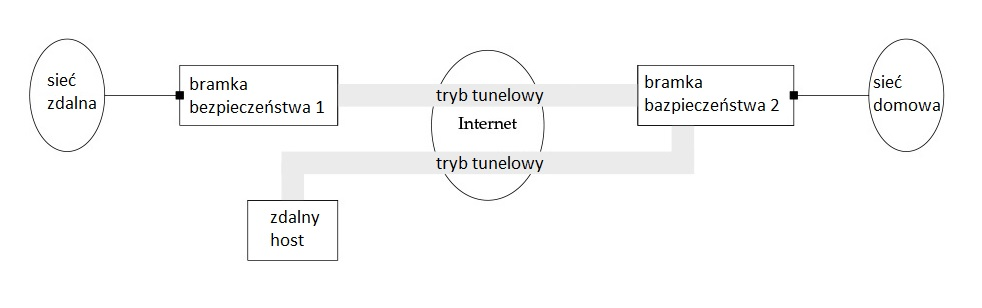
\includegraphics[width=10cm]{tryb_tunelowy_IPsec.jpg}
\caption{Tryb tunelowy IPsec}\label{IPsec}
\end{figure}
 
\quad Sieć zdalna jest połączona z siecią domową za pośrednictwem sieci tunelowej, bramki bezpieczeństwa 1 i bramki bezpieczeństwa 2. Funkcją bramek jest szyfrowanie, deszyfrowanie, zapobieganie ponownego odtwarzania wysyłanych pakietów i uwierzytelnianie. Z poziomu hostów bramki bezpieczeństwa i tunelowanie jest niewidoczne. Występują trzy metody uwierzytelnienie danych z udziałem protokołu bezpieczeństwa IPsec: wstępnie uzgodnione klucze, klucze prywatne i publiczne RSA oraz certyfikaty. Nagłówki uwierzytelniające dla trybu transportowego i tunelowego różnią się od siebie. Powszechny pakiet IP wchodzący w wyższą warstwę TCP składa się z: nagłówka IP, nagłówka TCP i danych użytkownika. Dla trybu transportowego nagłówek uwierzytelnienia dla IPsec składa się z: nagłówka IP, nagłówka uwierzytelniającego, nagłówka TCP i danych użytkownika. W tunelowym trybie nagłówek uwierzytelniający kopiuje część wewnętrzną nagłówka IP, która jest używana do utworzenia nowego zewnętrznego nagłówka IP. Nagłówek składa się z: zewnętrznego nagłówka IP, nagłówka uwierzytelniającego, wewnętrznego nagłówka IP, nagłówka TCP i danych użytkownika.

IPsec korzysta z protokołu Internet Key Exchange (IKE) w celu nawiązania i ustanowienie bezpiecznego połączenia między dwoma hostami lub zdalnego dostępu tunelowania VPN. Protokół IKE występuje w dwóch wersjach IKEv1 i IKEv2. Protokół IKEv1 można podzielić na dwie fazy, pierwsza w nich odpowiada za następujące funkcjonalności: algorytmy szyfrowania, algorytmy haszowania, protokół Diffiego-Hellmana oraz metodę uwierzytelniania.  Faza druga IKEv1 jest głównie używana do szyfrowania w protokole IPsec. Do szyfrowania wykorzystujemy algorytmy Data Encryption Standard (DES),  Triple DESo długości 168 bitów czy Advanced Encryption Standard (AES) o długości 128-256 bitów. Spośród wymienionych powyżej algorytmów DES zapewnia najniższe bezpieczeństwo danych, zaś AES o długości klucza 256 bitów największe bezpieczeństwo. Algorytmy haszujące zastosowane w protokole IPsec to: Secure Hash Algorithm (SHA) oraz Message Digest 5 (MD5). Protokół MD5 jest mniej bezpieczny niż algorytm SHA.
Kiedy używamy IPsec wraz z VPN przesyłane dane będą zabezpieczone podczas przesyłania, w celu uniemożliwienia atakującemu zdobycie jawnych danych.  Proces szyfrowania, który zapewnia poufność przesyłanych danych nie daje możliwości łatwej modyfikacji wrażliwych danych atakującemu.

Do stworzenia protokołu IPsec zrzeszenia bezpieczeństwa(Security Association AS) używanych jest kilka komponentów, które służą do przetwarzania ruchu tekstu jawnego, który jest chroniony i następnie przekształcany w tekst zaszyfrowany. Te same komponenty są używane do odszyfrowania danych. Protokół IPsec korzysta z trzech baz danych: 
\begin{itemize}
\item Baza danych zasad zabezpieczeń - Security Policy Database (SPD) określa jaki ruch ma być chroniony
\item Baza danych stowarzyszenia zabezpieczeń - Security Association Database (SAD) określa w jaki sposób ruch jest chroniony
\item Baza danych autoryzacji - Peer Authorization Database (PAD) zapewnia mechanizm wymuszający  politykę z oparciu o protokół IKE
\end{itemize}

\subsubsection{Secure Socket Tunneling protocol Based on VPN}
\quad Protokół SSTP umożliwia administratorom na ustanowienie tunelów poprzez główną sieć korporacyjną na Windows Serwer. Dzięki zredukowanie wymaganych kroków technicznych do utworzenia tunelów między organizacjami zyskujemy niższy koszt administracyjny. Brak dodatkowych zmian w infrastrukturze dla protokołu SSTP, gdyż podobnie jak w protokóle HTTPS jest obsługiwana zapora sieciowa i serwery proxy. Protokół SSTP wykorzystuje protokołu SSL do transportu ruchu sieciowego. SSL jest certyfikatem odpowiedzialnym za poświadczenie wiarygodności domeny bądź jej właściciela, co zapewnia bezpieczeństw szyfrowania danych. PPP to protokół połączenie punkt-punkt. Protokołem odpowiedzialnym za sterowanie transmisją jest TCP. 
Proces utworzenia połączenia wykorzystującego VPN między klientem, a serwerem przebiega w następujący sposób:
\begin{itemize}
\item klient ustanawia połączenie TCP z serwerem SSTP pomiędzy dynamicznie zaalokowanym portem TCP po stronie klienta SSTP, a portem TCP 443 na serwerze SSTP
\item klient SSTP wysyła wiadomość Witaj SSL świadczącą o chęci nawiązania połączenia SSL z serwerem SSTP
\item serwer SSTP wysyła do klienta cyfrowy certyfikat
\item klient SSTP sprawdza poprawność certyfikatu, wybiera metodę szyfrowania dla sesji SSL, generuje klucze i następnie szyfruje certyfikat serwera przy użyciu klucza publicznego
\item klient SSTP wysyła zaszyfrowany klucz sesji SSL do serwera SSTP
\item serwer SSTP odszyfrowuje zaszyfrowany klucz sesji SSL z wykorzystaniem klucza prywatnego; dalsza komunikacja klienta z serwerem jest zaszyfrowana wybraną metodą szyfrowania i odszyfrowywana kluczem sesji SSL
\item klient wysyła komunikat HTTP poprzez sesję SSL do serwera
\item klient ustala połączenie tunelowe z serwerem
\item klient SSTP ustala połączenie PPP z serwerem SSTP, które obejmuje uwierzytelnienie danych logowanie użytkownika wraz z uwierzytelnieniem PPP i ustawieniem konfiguracji ruchu IP
\item klient SSTP rozpoczyna proces ruchu sieciowego IP poprzez łącze PPP~\cite{SSTP}
\end{itemize}

\subsubsection{L2TP}
\quad Protokół tunelujący warstwy 2 (Layer 2 Tunneling Protocol L2TP) działa na warstwie łączy danych, która jest drugą w siedmio warstwowym modelu odniesienia łączenia systemów otwartych (OSI). Protokół ten nie zapewnia szyfrowania ani poufności danych, z tego powodu jest często używany z protokołem IPsec który zapewnia szyfrowanie i poufność danych. Protokół służy do komunikacji między klientem zwanym jako koncentrator dostępu L2TP(LAC) oraz serwerem nazywanym sieciowym serwerem L2TP (LNS). 
Protokół L2TP, który jest wykorzystywany do włączenie sieci VPN w Internecie jest rozszerzeniem protokołu PPTP. Powstał on w połączeniu protokołu firmy PPTP opracowanej przez Microsoft i L2F (przekierowywanie warstwy drugiej modelu OSI) firmy Cisco. Połączenie użytkownika domowego do sieci firmowej wykorzystujące protokół L2TP i połączenie internetowe przedstawiono w następujących krokach:
\begin{itemize}
\item zdalny użytkownik korzysta z analogowego połączenia telefonicznego lub łącza szerokopasmowego w celu zainicjowania połączenie PPP do dostawcy usług internetowych
\item sieć LAC akceptuje połączenie co prowadzi do ustanowienia połączenia PPP
\item w czasie gdy użytkownik końcowy i serwer nawiązują połączenie, koncentrator dostępu LAC rozpoczyna uwierzytelniania użytkownika metodą CHAP lub PAP
\item po pomyślnie ukończonym procesie uwierzytelnienia, połączenie użytkownika z serwerem LNS zostaje pomyślnie nawiązane; w przypadku niepomyślnego procesu uwierzytelnienie klient uzyskuje dostęp do Internetu jako normalny użytkownik
\item punkty końcowe tunelu (LAC i LNS) przed wysłaniem danych poprzez tunel uwierzytelniają się wzajemnie
\item po utworzeniu tunelu VPN korzystającego z protokołu L2TP połączenie między użytkownikiem, a siecią korporacyjną zostaje nawiązane 
\end{itemize}
Protokół L2TP jest protokołem sieci komputerowej wykorzystywanym przez dostawców internetowych do utworzenia wirtualnej sieci prywatnej między dwoma urządzeniami.~\cite{L2TP}

\newpage
\section{Systemy wbudowane}
\subsection{Budowa }
\paragraph{Rejestr} \mbox{} \\ % rejestr i rejsster specjalny
\paragraph{Pamięć} \mbox{} \\% nieulotne i ulotne
\paragraph{Porty wejścia/wyjścia} \mbox{} \\
\paragraph{Centralne jednostka obliczeniowa} \mbox{} \\
\paragraph{Dekoder instrukcji} \mbox{} \\
\paragraph{Jednostka arytmetyczno-logiczna ALU} \mbox{} \\
\paragraph{Rejestr SREG} \mbox{} \\
\paragraph{Zegar} \mbox{} \\
\paragraph{Magistrala} \mbox{} \\
\paragraph{Linie danych, adresowe i sterowania} \mbox{} \\

\subsection{Architektura systemów wbudowanych}
\quad Architekturę systemów wbudowanych możemy podzielić na architekturę zależną od struktury pamięci i zależną od typu instrukcji. Struktura pamięci : harwardzka, zmodyfikowana harwardzka i von-Neumanna. Typu instrukcji RISC i CISC.
\subsubsection{Architektura harwardzka}
\subsubsection{Zmodyfikowana architektura harwardzka}
\subsubsection{Architektura von-Neumanna}
\subsubsection{RISC - Recuded Instruction Set Computer}
\subsubsection{CISC - Complex Instruction Set Computer}

\newpage
\part{Część praktyczna}
\section{Aplikacja algorytmów kryptograficznych na systemie wbudowanym}
  ...
\subsection{Charakterystyka systemu wbudowanego}
\subsection{Szyfrowanie przy użyciu algorytmu DES}

!!!!!!!!!!!!!!!!!!!!!!!!!!!!!!!!!!!!!!!!!!!!!!!!!!!!!
!!!!!!!!!!!!!!!!!!!!!!  Przykład użycia algorytmu DES.
 
\begin{table}[H]
\centering
\begin{tabular}{|c|c|c|c|c|c|c|c|c|}
\hline
wiadomość & witaj :)\\
\hline
wiadomość w postaci heksadecymalnej & 77 69 74 61 6A 20 3A 29\\
\hline
klucz & 43 23 66 A3 6B BB 53 C1\\
\hline
\end{tabular}
\caption{Dane wejściowe algorytmu DES.}~\label{binary}
\end{table}

\begin{table}[H]
\centering
\begin{tabular}{|c|c|c|c|c|c|c|c|c|}
\hline
klucz & 4 & 3 & 2 & 3 & 6 & 6 & A & 3\\
\hline
klucz w postaci binarnej & 0100 & 001\textbf{1} & 0010 & 001\textbf{1} & 0110 & 011\textbf{0} & 1010 & 001\textbf{1}\\ 
\hline
numer bitu & 0-3 & 4-7 & 8-11 & 12-15 & 16-19 & 20-23 & 24-28 & 29-32\\
\hline
\hline
klucz & 6 & B & B & B & 5 & 3 & C & 1\\
\hline
klucz w postaci binarnej & 0110 & 101\textbf{1} & 1011 & 101\textbf{1} & 0101 & 001\textbf{1} & 1100 & 000\textbf{1}\\
\hline
numer bitu & 33-36 & 37-40 & 41-44 & 45-48 & 49-52 & 53-56 & 57-60 & 61-64\\
\hline
\end{tabular}
\caption{Klucz w postaci binarnej.}~\label{klucz_to_binary}
\end{table}

Po przekształceniu heksadecymalnego klucza do postaci binarnej usuwamy bit parzystości z 64 bitowego bloku czyli 8, 16, 24, 32, 40, 48, 56 i 64 bit. W tabeli~\ref{klucz_to_binary} bit parzystości oznaczono pogrubioną kursywą.

Następnie z wykorzystaniem tabeli~\ref{per_klucza} dokonujemy przestawienie bitów klucza, odszukano bit 57 klucza, który wynosi 0 i wpisano do nowo utworzonej tabeli ~\ref{tabela_podstawienia} w lewym górnym rogu. W tak przedstawiony sposób dokonano translacji dla dalszych bitów klucza, a wynik przedstawiono w tabeli~\ref{tabela_podstawienia}.

\begin{table}[H]
\centering
\begin{tabular}{|c|c|c|c|c|c|c|c|c|c|c|c|c|c|c|c|c|}
\hline
permutacja klucza & 57 & 49 & 41 & 33 & 25 & 17 & 9 & 1 & 58 & 50 & 42 & 34 & 26 & 18 & &\\
\hline
numer bitu & 0 & 1 & 2 & 3 & 4 & 5 & 6 & 7 & 8 & 9 & 10 & 11 & 12 & 13 & 14 & 15\\
\hline
klucz binarny & 0 & 1 & 0 & 0 & 0 & 0 & 1 & 1 & 0 & 0 & 1 & 0 & 0 & 0 & 1 & 1\\
\hline
klucz po permutacji & 1 & 1 & 0 & 1 & 0 & 1 & 0 & 0 & 0 & 0 & 1 & 1 & 1 & 1 &&\\

\hline
\hline
permutacja klucza & 10 & 2 & 59 & 51 & 43 & 35 & 27 & 19 & 11 & 3 & 60 & 52 & 44 & 36 &&\\
\hline
numer bitu & 16 & 17 & 18 & 19 & 20 & 21 & 22 & 23 & 24 & 25 & 26 & 27 & 28 & 29 & 30 & 31\\
\hline
klucz binarny & 0 & 1 & 1 & 0 & 0 & 1 & 1 & 0 & 1 & 0 & 1 & 0 & 0 & 0 & 1 & 1\\
\hline 
klucz po permutacji & 1 & 0 & 0 & 1 & 1 & 0 & 0 & 0 & 0 & 0 & 0 & 0 & 1 & 1 &&\\

\hline
\hline
permutacja klucza & 63 & 55 & 47 & 39 & 31 & 23 & 15 & 7 & 62 & 54 & 46 & 38 & 30 & 22 &&\\
\hline
numer bitu & 32 & 33 & 34 & 35 & 36 & 37 & 38 & 39 & 40 & 41 & 42 & 43 & 44 & 45 & 46 & 47 \\
\hline
klucz binarny & 0 & 1 & 1 & 0 & 1 & 0 & 1 & 1 & 1 & 0 & 1 & 1 & 1 & 0 & 1 & 1 \\
\hline
klucz po permutacji & 1 & 1 & 1 & 1 & 1 & 0 & 1 & 1 & 0 & 1 & 1 & 1 & 1 & 1 &&\\

\hline
\hline
permutacja klucza & 14 & 6 & 61 & 53 & 45 & 37 & 29 & 21 & 13 & 5 & 28 & 20 & 12 & 4 &&\\
\hline
numer bitu & 48 & 49 & 50 & 51 & 52 & 53 & 54 & 55 & 56 & 57 & 58 & 59 & 60 & 61 & 62 & 63\\
\hline
klucz binarny & 0 & 1 & 0 & 1 & 0 & 0 & 1 & 1 & 1 & 1 & 0 & 0 & 0 & 0 & 0 & 1\\
\hline 
klucz po permutacji & 1 & 1 & 0 & 0 & 0 & 0 & 0 & 1 & 0 & 0 & 0 & 0 & 0 & 0 &&\\
\hline
\end{tabular}
\caption{Klucz w postaci binarnej.}~\label{tabela_podstawienia}
\end{table}


Klucz po permutacji z postawi 64 bitowej redukuje się do postaci 56 bitowej i dzieli na dwie części: prawą i lewą. 

\begin{table}[H]
\centering
\begin{tabular}{|c|}
\hline
1101 0100 0011 1110 0110 0000 0011\\
\hline
1111 1011 0111 1111 0000 0100 0000\\
\hline
\end{tabular}
\caption{Obliczony klucz w postaci 56 bitowej.}
\end{table}

* przesunięcie bitowe klucza o 1 w lewo
\begin{table}[H]
\centering
\begin{tabular}{|c|}
\hline
1010 1000 0111 1100 1100 0000 0111\\
\hline
1111 0110 1111 1110 0000 1000 0001\\
\hline
\end{tabular}
\caption{Obliczony klucz w postaci 56 bitowej.}
\end{table}

* Permutacja kompresji klucza DES (transpozycja tabeli~\ref{per_kompresji} kompresji klucza z 56 bitami przesuniętego klucza.

\begin{table}[H]
\centering
\begin{tabular}{ | p{3cm} | p{1.7cm} | p{1.7cm} | p{1.7cm} | p{1.7cm} | p{1.7cm} | p{1.7cm} |}
\hline
permutacja kompresji DES & 14 17 11 24  & 1 5 3 28 &  15 6 21 10 & 23  19 12 4 & 26 8 16 7 & 27 20 13 2\\ \hline
bitowy klucz 56bitowy po permutacji & 1110 & 1111 & 0001 & 0000 & 1000 & 1010 \\ \hline
heksadecymalny klucz 56bitowy po permutacji & E & F & 1 & 0 & 8 & A\\
\hline \hline
permutacja kompresji DES & 41 52 31 37 & 47 55 30 40 & 51 45 33 48 & 44 49 39 56 & 34 53 46 42 & 50 36 29 32\\ \hline
bitowy klucz 56bitowy po permutacji & 0010 & 0011 & 0000 & 0111 & 1001 & 0011\\ \hline
heksadecymalny klucz 56bitowy po permutacji & 2 & 3 & 0 & 7 & 9 & 3\\ 
\hline
\end{tabular}
\caption{Obliczony klucz w postaci 56 bitowej.}
\end{table}

* Obliczony klucz w pierwszym etapie to EF108A230793.

!!!!!!!!!! Obliczenie permutacji początkowej 

\begin{table}[H]
\centering
\begin{tabular}{|c|c|c|c|c|c|c|c|c|}
\hline
wiadomość heksadecymalna & 7 & 7 & 6 & 9 & 7 & 4 & 6 & 1\\ \hline
wiadomość binarna & 0111 & 0111 & 0110 & 1001 & 0111 & 0100 & 0110 & 0001\\ \hline
numer bitu & 1-4 & 5-8 & 9-12 & 13-16 & 17-20 & 21-24 & 25-28 & 29-32\\ \hline
wiadomość heksadecymalna & 6 & A & 2 & 0 & 3 & A & 2 & 9\\ \hline
wiadomość binarna & 0110 & 1010 & 0010 & 0000 & 0011 & 1010 & 0010 & 1001\\ \hline
numer bitu & 33-36 & 37-40 & 41-44 & 44-48 & 49-52 & 53-56 & 57-60 & 61-64\\ \hline
\end{tabular}
\caption{Wiadomość przedstawiona w postaci binarnej i heksadecymalnej.}
\end{table}


\begin{table}[H]
\centering
\begin{tabular}{|c|c|c|c|c|c|c|c|c|c|}
\hline
wiadomość binarna po permutacji & 0001 & 1111 & 0100 & 0101 & 0000 & 0101 & 1000 & 1011\\ \hline
wiadomość heksadecymalna po permutacji & 1 & F & 4 & 5 & 0 & 5 & 8 & B\\ \hline
wiadomość binarna po permutacji & 0000 & 0000 & 1111 & 1111 & 1101 & 0010 & 0101 & 0001\\ \hline
wiadomość heksadecymalna po permutacji & 0 & 0 & F & F & D & 2 & 5 & 1\\ \hline

\end{tabular}
\caption{Transpozycja wiadomości w postaci binarnej z tabelą permutacji początkowej.}
\end{table}



Lewa strona wiadomości to L = 1F45058B, prawa strona P = 00FFD251. 
Dla rundy pierwszej algorytmu lewą stroną wiadomości zostaje prawa część wiadomości, natomiast prawą część wiadomości obliczamy następująco:
*  prawa część wiadomości podlega transpozycji zgodnie z tabelą permutacji rozszerzenia 
* operacja XOR wiadomości otrzymanej w wyniku transpozycji z obliczonym kluczem EF108A230793.



* prawa część wiadomości podlega transpozycji zgodnie z tabelą permutacji rozszerzenia dając wynik w tabeli poniżej.
\begin{table}[H]
\begin{tabular}{|c|c|}
\hline
prawa część wiadomości & 00FFD251\\ \hline
& 0000 0000 1111 1111 1101 0010 0101 0001\\ \hline
permutacja rozszerzenia & 100000 000001 011111 111111 111010 100100 001010 100010\\ \hline
\end{tabular}
\end{table}


\begin{table}[H]
\begin{tabular}{|c|c|}
\hline
wiadomość & 100000 000001 011111 111111 111010 100100 001010 100010\\ \hline
klucz & 111011 110001 000010 001010 001000 110000 011110 010011\\ \hline
XOR & 011011 110000 011101 110101 110010 010100 010100 110001\\ 
\hline
\end{tabular}
\caption{XOR wiadomości po permutacji rozszerzenia z kluczem.}\label{xor}
\end{table}

!!!!!!!! Podstawienie w S-blokach

W tabeli

Wynik operacji XOR z tabeli ~\ref{xor} podzielono na S1 = 011011, S2 = 110000, S3 = 011101, S4 = 110101, S5 = 110010, S6 = 010100, S7 = 010100 i S8 = 110001. Wartości S bloków odczytano z użyciem tabeli~\ref{s_bloki}. Pierwszy w ostatni bit bloku oznacza rząd z tabeli~\ref{s_bloki} S-bloków, wartości 00 oznaczają wiersz 0, 01 oznaczają wiersz 1, 10 oznaczają wiersz 2, zaś 11 oznaczają wiersz 3. Dla wartości S1 pierwszy i ostatni bit bloku S1 = 01, co znaczy korzystanie z wiersza 1 S bloku 1. Następnie cztery bity między 1-5 bitem zmieniono na wartość decymalną. Dla S1 postać binarna 1101 wynosi 13 w postaci decymalnej, z tabeli~\ref{s_bloki} odczytujemy z wiersza 1, kolumny 13 wartość  5, więc S1 = 9. W sposób analogiczny odczytano pozostałe wartości S-bloków, które przedstawiono poniżej:
 
S1 = 5, S2 = 12, S3 = 15, S4 = 5, S5 = 9, S6 = 3, S7 = 9,S8 = 15.

\begin{table}[H]
\centering
\begin{tabular}{|c|c|c|c|c|c|c|c|c|} 
\hline
decymalnie &5 &12& 15& 5& 9& 3& 9& 15\\ \hline
binarnie & 0101& 1100& 1111& 0101& 1001& 0011& 1001& 1111\\ \hline
numer bitu &1-4 &5-8& 9-12& 13-16& 17-20& 21-24& 25-28& 29-32\\ \hline
\end{tabular}
\end{table}



Dokonujemy transpozycji wyjścia S bloku z tabelą permutacji P-bloku~\ref{blok_P} w wyniku czego otrzymano: 1010 1111 0010 1011 1011 1001 0011 0111. Otrzymaną wartość poddano operacji XOR z lewą połową wiadomości (1F45058B), co przedstawiono jako (1010 1111 0010 1011 1011 1001 0011 0111) $/oplus$ (0001 1111 0100 0101 0000 0101 1000 1011) = 1011 0000 0110 1110 1011 1100 1011 1100, co w postaci heksadecymalnej daje wartość B06EBCB3.



Wartość prawej strony rundy pierwszej wynosi B06EBCB3. 

\subsection{Implementacja algorytmów szyfrujących}
\subsubsection{Implementacja szyfru Cezara}
\subsubsection{Implementacja szyfru DES}
\subsection{Wyniki implementacji algorytmów szyfrujących} 
\newpage
\section{Wnioski}
\section{Podsumowanie}
%3. Później w podsumowaniu warto nawiązać do Celu i zakresu podkreślając co zostało zrobione, a co np. nie z podaniem powodów.
\newpage
\begin{thebibliography}{99}

\bibitem{PPTP} D. Stoddard i T.M. Thomas,
\emph{
Cover image for Network Security First-Step, Second Edition
Network Security First-Step, Second Edition},
Cisco Press, 12.2011, chapter 6

\bibitem{SSH} A. Lockhart,
\emph{Network Security Hacks},
O'Reilly Media Inc., 04.2004, chapter 6

\bibitem{SSTP} J. Savill,
\emph{The Complete Guide to Windows Server 2008},
Addison-Wesley Professional, 10.2008, chapter 8

\bibitem{L2TP} S. Malik,
\emph{Cover image for Network Security Principles and Practices
Network Security Principles and Practices},
Cisco Press, 10.2002

\bibitem{DES} J. Wiley,
\emph{Information Security: Principles and Practice,2nd Edition},
M. Stamp, 05.2011, chapter 3

\bibitem{IDEAA} N. Hoffman,
\emph{Article in Cryptologia: A simplified IDEA algorithm},
Department of Mathematics, Northern Kentucky University, March 2007, str 143-151

\bibitem{IDEA} Tingting CuiHuaifeng ChenLong WenMeiqin Wang,
\emph{Cryptography and Communications: Statistical integral attack on CAST-256 and IDEA}, January 2018, Volume 10

\bibitem{RSA}
\emph{Information Security: Principles and Practice, 2nd Edition},

\bibitem{DH} C. Chebbi
\emph{Advanced Infrastructure Penetration Testing},
Packt Publishing, 02.2018

% NIE PODAWAC TEJ LITERATURY ----
%\bibitem{stream_cipher}O. Santos and J. Stuppi,
%\emph{
%Applied Cryptography: Protocols, Algorithms and Source Code in C, 20th Anniversary Edition},
%John Wiley and Sons, 03.2015, chapter 16

\end{thebibliography}
\newpage
\listoffigures
\addcontentsline{toc}{section}{Literatura}
\addcontentsline{toc}{section}{Spis rysunków}

\end{document}
